\documentclass[12pt,preprint, authoryear]{article}

\pagestyle{plain}

\usepackage{lmodern}
%%%% My spacing
\usepackage{setspace}
\setstretch{1.25}
\DeclareMathSizes{10}{12}{8}{8}

% Wrap around which gives all figures included the [H] command, or places it "here". This can be tedious to code in Rmarkdown.
\usepackage{float}
\let\origfigure\figure
\let\endorigfigure\endfigure
\renewenvironment{figure}[1][2] {
    \expandafter\origfigure\expandafter[H]
} {
    \endorigfigure
}

\let\origtable\table
\let\endorigtable\endtable
\renewenvironment{table}[1][2] {
    \expandafter\origtable\expandafter[H]
} {
    \endorigtable
}


\usepackage{ifxetex,ifluatex}
\usepackage{fixltx2e} % provides \textsubscript
\ifnum 0\ifxetex 1\fi\ifluatex 1\fi=0 % if pdftex
  \usepackage[T1]{fontenc}
  \usepackage[utf8]{inputenc}
\else % if luatex or xelatex
  \ifxetex
    \usepackage{mathspec}
    \usepackage{xltxtra,xunicode}
  \else
    \usepackage{fontspec}
  \fi
  \defaultfontfeatures{Mapping=tex-text,Scale=MatchLowercase}
  \newcommand{\euro}{€}
\fi

\usepackage{amssymb, amsmath, amsthm, amsfonts}

\usepackage[round]{natbib}
\bibliographystyle{natbib}
\def\bibsection{\section*{References}} %%% Make "References" appear before bibliography
\usepackage{longtable}
\usepackage[left=2cm, right=2cm, top=20mm, bottom=4cm, top=2.5cm, includefoot]{geometry}
\usepackage{fancyhdr}
\usepackage[bottom, hang, flushmargin]{footmisc}
\usepackage{graphicx}
\numberwithin{equation}{section}
\numberwithin{figure}{section}
\numberwithin{table}{section}
\setlength{\parindent}{0cm}
\setlength{\parskip}{1.3ex plus 0.5ex minus 0.3ex}
\usepackage{textcomp}
\renewcommand{\headrulewidth}{0pt}

\usepackage{array}
\newcolumntype{x}[1]{>{\centering\arraybackslash\hspace{0pt}}p{#1}}

%%%%  Remove the "preprint submitted to" part. Don't worry about this either, it just looks better without it:

\makeatletter
\def\ps@pprintTitle{%
  \let\@oddhead\@empty
  \let\@evenhead\@empty
  \let\@oddfoot\@empty
  \let\@evenfoot\@oddfoot
}

\usepackage{hyperref}
\hypersetup{breaklinks=true,
            bookmarks=true,
            colorlinks=true,
            citecolor=blue,
            urlcolor=blue,
            linkcolor=blue,
            pdfborder={0 0 0}}
						
\urlstyle{same}  % don't use monospace font for urls
\setlength{\parindent}{0pt}
\setlength{\parskip}{6pt plus 2pt minus 1pt}
\setlength{\emergencystretch}{3em}  % prevent overfull lines
\setcounter{secnumdepth}{5}

%%% Use protect on footnotes to avoid problems with footnotes in titles
\let\rmarkdownfootnote\footnote%
\def\footnote{\protect\rmarkdownfootnote}
\IfFileExists{upquote.sty}{\usepackage{upquote}}{}

%%% Include extra packages specified by user

%%% Change title format to be more compact
\usepackage{titling}

% Create subtitle command for use in maketitle
%\newcommand{\subtitle}[1]{
  %\posttitle{
    %\begin{center}\large#1\end{center}
    %}
%}

\setlength{\droptitle}{-1em}
\title{Online Community Engagement: Validating Classification Methodologies on
StackExchange Fora}
\pretitle{\vspace{\droptitle}\centering\huge}
\posttitle{\par\vskip 0.5em}
\author{Bradley Carruthers, Candidate Number: 10140}
\preauthor{\centering\large}
\postauthor{\par}
\predate{\centering\large}
\postdate{\par}
\date{3 May 2019}

\usepackage{color}
\usepackage[usenames,dvipsnames,svgnames,table]{xcolor}
\usepackage{hyperref}
\hypersetup{
     colorlinks   = true,
     citecolor    = gray
}

\usepackage{tocloft}

\renewcommand{\cftsubsecfont}{\normalfont\hypersetup{linkcolor=black}}
\renewcommand{\cftsubsecafterpnum}{\hypersetup{linkcolor=black}}

\begin{document}

%________________________
% Header and Footers
%%%%%%%%%%%%%%%%%%%%%%%%%%%%%%%%%
\pagestyle{fancy}
\chead{}
\rhead{}
\lfoot{}
\rfoot{} 
\lhead{}
%\rfoot{\footnotesize Page \thepage\ } % "e.g. Page 2"
\cfoot{\footnotesize \thepage\\}

%\setlength\headheight{30pt} 
%%%%%%%%%%%%%%%%%%%%%%%%%%%%%%%%%
%________________________

%\headsep 35pt % So that header does not go over title

%\begin{frontmatter}

\pagenumbering{roman}

\maketitle
\thispagestyle{empty}

%\author{Bradley Carruthers, Candidate Number: 10140}
%\date{3 May 2019}

%\end{frontmatter}

\clearpage

\setcounter{page}{1}

\section*{Abstract}

The world wide web and the technologies that have accompanied it have
given us the exceptional ability to comment on, engage with and question
the world. While much attention has been given to identifying
high-quality answers online, less consideration has been afforded to how
we can improve our questions, which can be particularly beneficial for
online question-answering communities where subject matter is often
technical and expert resources are scarce.

One avenue to address issues of limited resources and information
overload on online communities is to nudge questioners to enhance the
``signal'' of their questions before adding demand to a community, and
this can be achieved by modeling and predicting positive community
engagement for questions. The research presented here takes the first
step towards this objective by building on and validating work already
done on question quality and community engagement in online fora. By
analysing question content from a diverse range of online communities, I
am able to shed light on optimal thresholds for labeling positive and
negative community engagement, improving upon work done in this area.

\newpage

\renewcommand{\contentsname}{Contents}
\hypersetup{linkcolor=black}
\tableofcontents
\newpage
\hypersetup{linkcolor=black}
\listoftables
\newpage
\hypersetup{linkcolor=black}
\listoffigures
\hypersetup{linkcolor=black}
\newpage

\pagenumbering{arabic}

\renewcommand{\vec}[1]{\mathbf{#1}}

\newgeometry{left=2cm, right=2cm, top=2.5cm, bottom=4cm}

\section{\texorpdfstring{Introduction
\label{Intro}}{Introduction }}\label{introduction}

The advent of the internet and the interpersonal communication
technologies that have evolved from it have given us an unprecedented
level of connection and potential interaction with the world. Every day,
billions of individuals engage online not only with people they know,
but with complete strangers from across the globe. A considerable
challenge with there online interactions is widespread incivility, with
substantial work being devoted to understanding and addressing this
(Gervais, 2015; Berry and Taylor, 2017).

Online social question-answer (Q\&A) fora present environments where
community engagement (up-votes, answers, comments) and community
guidelines should mitigate many of the issues experienced by other more
provocative online platforms, yet these communities are not without
issues of their own. Certain fora, such as popular Massive Online Open
Courses (MOOCs), suffer from ``information overload'' where the degree
of off-topic activity and discussion makes it difficult for answerers to
find and engage with questions they \emph{can} answer, let alone review
all questions in the community.

Scarcity of expert resources seems to be a persistent problem in social
Q\&A systems, and thus the rationale for this research is to eventually
tackle question-formulation before they enter a community and place
demand on expert resources. One approach to achieve this would be to
build a classification model that can predict positive community
engagement with questions, and provide this information to questioners
so that they can be nudged into formulating a question that will better
received by a community (improving the "signal'' of their question).

The broad research question is therefore the following:

\begin{center}
\emph{To what extent can we capture positive community engagement with questions on online Q\&A communities?}
\end{center}

Here, positive community engagement is defined as constructive, amicable
interactions with user questions through answers, comments, votes, edits
and so on. One assumption made is that questions are heterogeneous in
that they have varying levels of ``quality'' which evoke either positive
and negative community reaction.

The research presented here is but an initial step in the ultimate goal
of classifying user questions and serves to build on methodologies and
approaches already taken to measure question quality/community
engagement. In this paper I analyse a diverse range of questions in fora
from the family of Q\&A communities, StackExchange. I use a metric for
community engagement to label questions as ``good'' and ``bad''
(receiving positive and negative community engagement respectively) and
find more optimal thresholds for this labeling by calculating similarity
metrics and linguistic differences across good/bad samples.

I now move onto a brief discussion of previous work in this field. This
is followed by descriptions of the datasets used, pre-processing steps
taken as well as exploratory analysis. I then discuss the methodology
for measuring community engagement with a specifically defined variable,
I present and discuss the results and lastly I make some concluding
remarks.

\section{Previous work}\label{previous-work}

Much work has gone into investigating online Q\&A communities. Research
has looked at answer quality (Jeon \emph{et al.}, 2006; Shah and
Pomerantz, 2010; Tian, Zhang and Li, 2013), behaviour of community
experts (Riahi \emph{et al.}, 2012; Sung, Lee and Lee, 2013) and
question-asker satisfaction (Liu, Bian and Agichtein, 2008). Also, a
common framework for engagement in Q\&A communities is the optimisation
of matching questions and community experts (Li and King, 2010; Li, King
and Lyu, 2011; Zhou, Lyu and King, 2012; Shah \emph{et al.}, 2018), or
recommending questions in line with answerers' interests (Wu, Wang and
Cheng, 2008; Qu \emph{et al.}, 2009; Szpektor, Maarek and Pelleg, 2013).

I choose to focus on questions, not only because they have received far
less attention in the literature, but because question quality impacts
answer quality (Agichtein \emph{et al.}, 2008) and because they are
trivially the initial touch-point of a community/questioner interaction.
It is highly likely therefore that increasing positive community
engagement will improve how these communities function and evolve.

Since community engagement and question quality can be seen as two sides
of the same coin (``good'' questions leading to favourable community
engagement), this research corresponds to a body of work on capturing
question quality in online question-answer communities which I briefly
discuss next. Note that while I consider community engagement a more
accurate definition of what the following literature measures, I refer
to ``question quality'' instead of community engagement to aid the
discussion.

Recent work (Agichtein \emph{et al.}, 2008; Bian \emph{et al.}, 2009; Li
\emph{et al.}, 2012) attempted to model question quality using
\href{http://answers.yahoo.com}{Yahoo! Answers}, however this dataset
lacks objective and definitive measures for question quality. The data
that I will be using on the other hand is richer in that there a
numerous proxies for question quality/community engagement available for
large sets of observations. Most importantly, these variables are
derived directly from the data rather than labeled manually, which
enables a more objective, automatic and principled characterisation of
the variable of interest.

One paper that made strides in classifying and predicting what they
assume to be question quality is Ravi \emph{et al.} (2014). Using latent
topics extracted from Latent Dirichlet Allocation models on question
content, they predict ``question quality'' with accuracy levels of 72\%
for the computer coding StackExchange community, StackOverflow.

Ravi \emph{et al.} (2014) decide on using a question's \texttt{Score} as
an indicator of question quality. I question this assumption and put
forth the notion that a question's \texttt{Score} better characterises
community engagement, since I believe it is difficult to define
``quality'' subjectively owing to communities valuing different facets
of questions (i.e.~closed-end for natural sciences or
discussion-promoting in the social sciences). I thus characterise it as
such and also use it as a response variable. This brings me to the aim
of this paper, which is to critique and build on how to use the
\texttt{Score} variable to label questions as attracting positive or
negative community engagement.

\newpage

\section{Data}\label{data}

\subsection{StackExchange Communities}\label{stackexchange-communities}

The data I use for this analysis are question-content text from the
family of online Q\&A communities,
\href{https://stackexchange.com/sites\#traffic}{StackExchange}. There
are more than 170 diverse StackExchange fora ranging from
science-fiction world building to bicycles to quantum computing, with
all the data publicly available in compressed XML files at
\href{http://archive.org/download/stackexchange}{archive.org}.

I chose to use the 8 largest datasets that my local machine could
handle, details of which are displayed below in table \ref{tab:fora}.

\renewcommand{\thetable}{\arabic{table}}

\footnotesize

\begin{longtable} {@{} cccp{12cm} @{}}
\caption{\textbf{Dataset Details}}
\label{tab:fora}\\ \hline \hline
Forum & Questions & Answers & Description \\ 
\hline
Buddhism & 5.7k & 19k & Discussions on Buddhist philosophy, teaching and practice \\
Economics & 7.7k & 9.9k & For those studying, teaching, researching and applying economics/econometrics \\
Fitness & 8.2k & 16k & Q\&A for athletes, trainers and physical fitness professionals \\ 
Health & 5.6k & 4.5k & For professionals in the medical and allied health fields \\ 
Interpersonal & 3.1k & 13k & Q\&A for anyone wanting to improve their interpersonal skills \\ 
Linguistics & 7k & 11k & Community for professional linguists and those interested in linguistic research \\
Outdoors & 4.9k & 12k & A forum for nature-enthusiasts \\ 
Spanish & 6.4k & 14k & Q\&A for Spanish language linguists, teachers, students and enthusiasts  \\
\hline \hline
\end{longtable}\begin{center} Source: Own calculations in R.\end{center}

\normalsize

For each forum, the following data is available per post in a
\texttt{Posts.xml} file:

\setstretch{0.65}

\begin{itemize}
\item
  \texttt{Id}: An identity variable for a post (chronological)
\item
  \texttt{PostTypeId}: Indicates if a post is a question (==1) or answer
  (==2)
\item
  \texttt{ParentId}: Indicates which question an answer belongs to
  (answers only)
\item
  \texttt{AcceptedAnswerId}: Indicates which answer the question-asker
  selects as accepted (questions only)
\item
  \texttt{CreationDate}: Indicates the date a post was originally made
\item
  \texttt{Score}: The difference between up-votes and down-votes for a
  post
\item
  \texttt{ViewCount}: The number of times a post has been viewed (not
  just site-registered users)
\item
  \texttt{Body}: Main post content
\item
  \texttt{OwnerUserId}: Indicates the user ID of a post's owner
\item
  \texttt{LastEditorUserId}: Indicates the user ID of the last user to
  edit a post
\item
  \texttt{LastEditDate}: Indicates the date a post was last edited
\item
  \texttt{LastActivityDate}: Indicates the date that there was last
  activity on the post (not including views)
\item
  \texttt{Title}: Post title (questions only)
\item
  \texttt{Tags}: Collection of tags linked when a question is made
  (questions only)
\item
  \texttt{AnswerCount}: Number of answers a question receives (questions
  only)
\item
  \texttt{CommentCount}: Number of comments a post receives
\item
  \texttt{FavoriteCount}: Number of times users favourite a question
  (questions only)
\item
  \texttt{ClosedDate}: A date variable indicating if a question was
  closed (questions only)
\end{itemize}

\setstretch{1.25}

This analysis will only use the \texttt{PostTypeId}, \texttt{Score},
\texttt{ViewCount} and \texttt{Body} variables.

\subsection{\texorpdfstring{Noteworthy elements
\label{noteworthy}}{Noteworthy elements }}\label{noteworthy-elements}

It is worth discussing the functioning of StackExchange sites in general
to more thoroughly understand the data. Questions across fora are
publicly available viewable by anyone on the internet, but posting a
question on forum requires email registration with the forum. After
registering, users start with 1
reputation\footnote{https://meta.stackexchange.com/questions/7237/how-does-reputation-work}.
The reputation levels that are key to this analysis are:

\setstretch{0.65}

\begin{itemize}
\item
  15: Gives you the ability to ``up-vote'' questions and answers
\item
  50: You can comment on questions and answers
\item
  125: You can ``down-vote'' questions and answers
\item
  2000: You can edit any question or answer.
\end{itemize}

\setstretch{1.25}

A number of methodological issues arise from how the sites operate.
Firstly, owing to all questions being open to the public, many people
may view questions without the ability to vote and thus still contribute
to the \texttt{ViewCount} variable. Additionally, the asymmetries for
privileges of up-voting and down-voting lead to a \texttt{Score}
variable that is highly negatively skewed, making it appear that there
are more ``good'' questions versus ``bad'' ones. Lastly, a major
confounding factor is the editing of questions, not only by original
posters, but also by anyone with 2000 reputation. This complicates much
of the engagement between question-askers and communities because no
data is available on the timing of answers, comments, votes, views etc.
in relation to question edits.

\subsection{Preprocessing and Exploratory
Analysis}\label{preprocessing-and-exploratory-analysis}

The entire analysis of the data was done with the statistical software
package \href{https://cran.r-project.org}{\texttt{R}} and a link to the
full code used in the analysis can be found
\href{https://github.com/BCallumCarr/msc-lse-thesis/tree/master/01-r-code}{here}.
After downloading and decompressing the data on the 8 selected forums, I
used the \texttt{R} functions \texttt{xmlParse} and \texttt{xmlToList}
from the \texttt{XML} package to parse and load the data into an
\texttt{R} tibble from the \texttt{tidyverse} \texttt{R} package. Some
regular expression work was needed to clean up the HTML text in
questions from the \texttt{Body} variable. The \texttt{PostTypeId}
variable was then used to separate out the question and answer posts,
and finally the descriptive bar graphs in figure \ref{fig:desc} were
created using \texttt{ggplot2}.

In figure \ref{fig:desc}, we see that average \texttt{Score} and
\texttt{ViewCount} per question vary substantially across fora.
Questions on the Interpersonal and Outdoors fora have average
\texttt{Scores} of approximately 17 and 11 respectively, compared to
around 3 or 4 for the other fora. Interpersonal also has a significantly
higher average \texttt{ViewCount} at approximately 4400 views per
question followed by Fitness, Outdoors and Spanish which all have an
average of around 3000.

\renewcommand{\thefigure}{\arabic{figure}}

\footnotesize

\begin{figure}
\caption{\textbf{Fora Descriptive Statistics}}
\label{fig:desc}

\begin{center}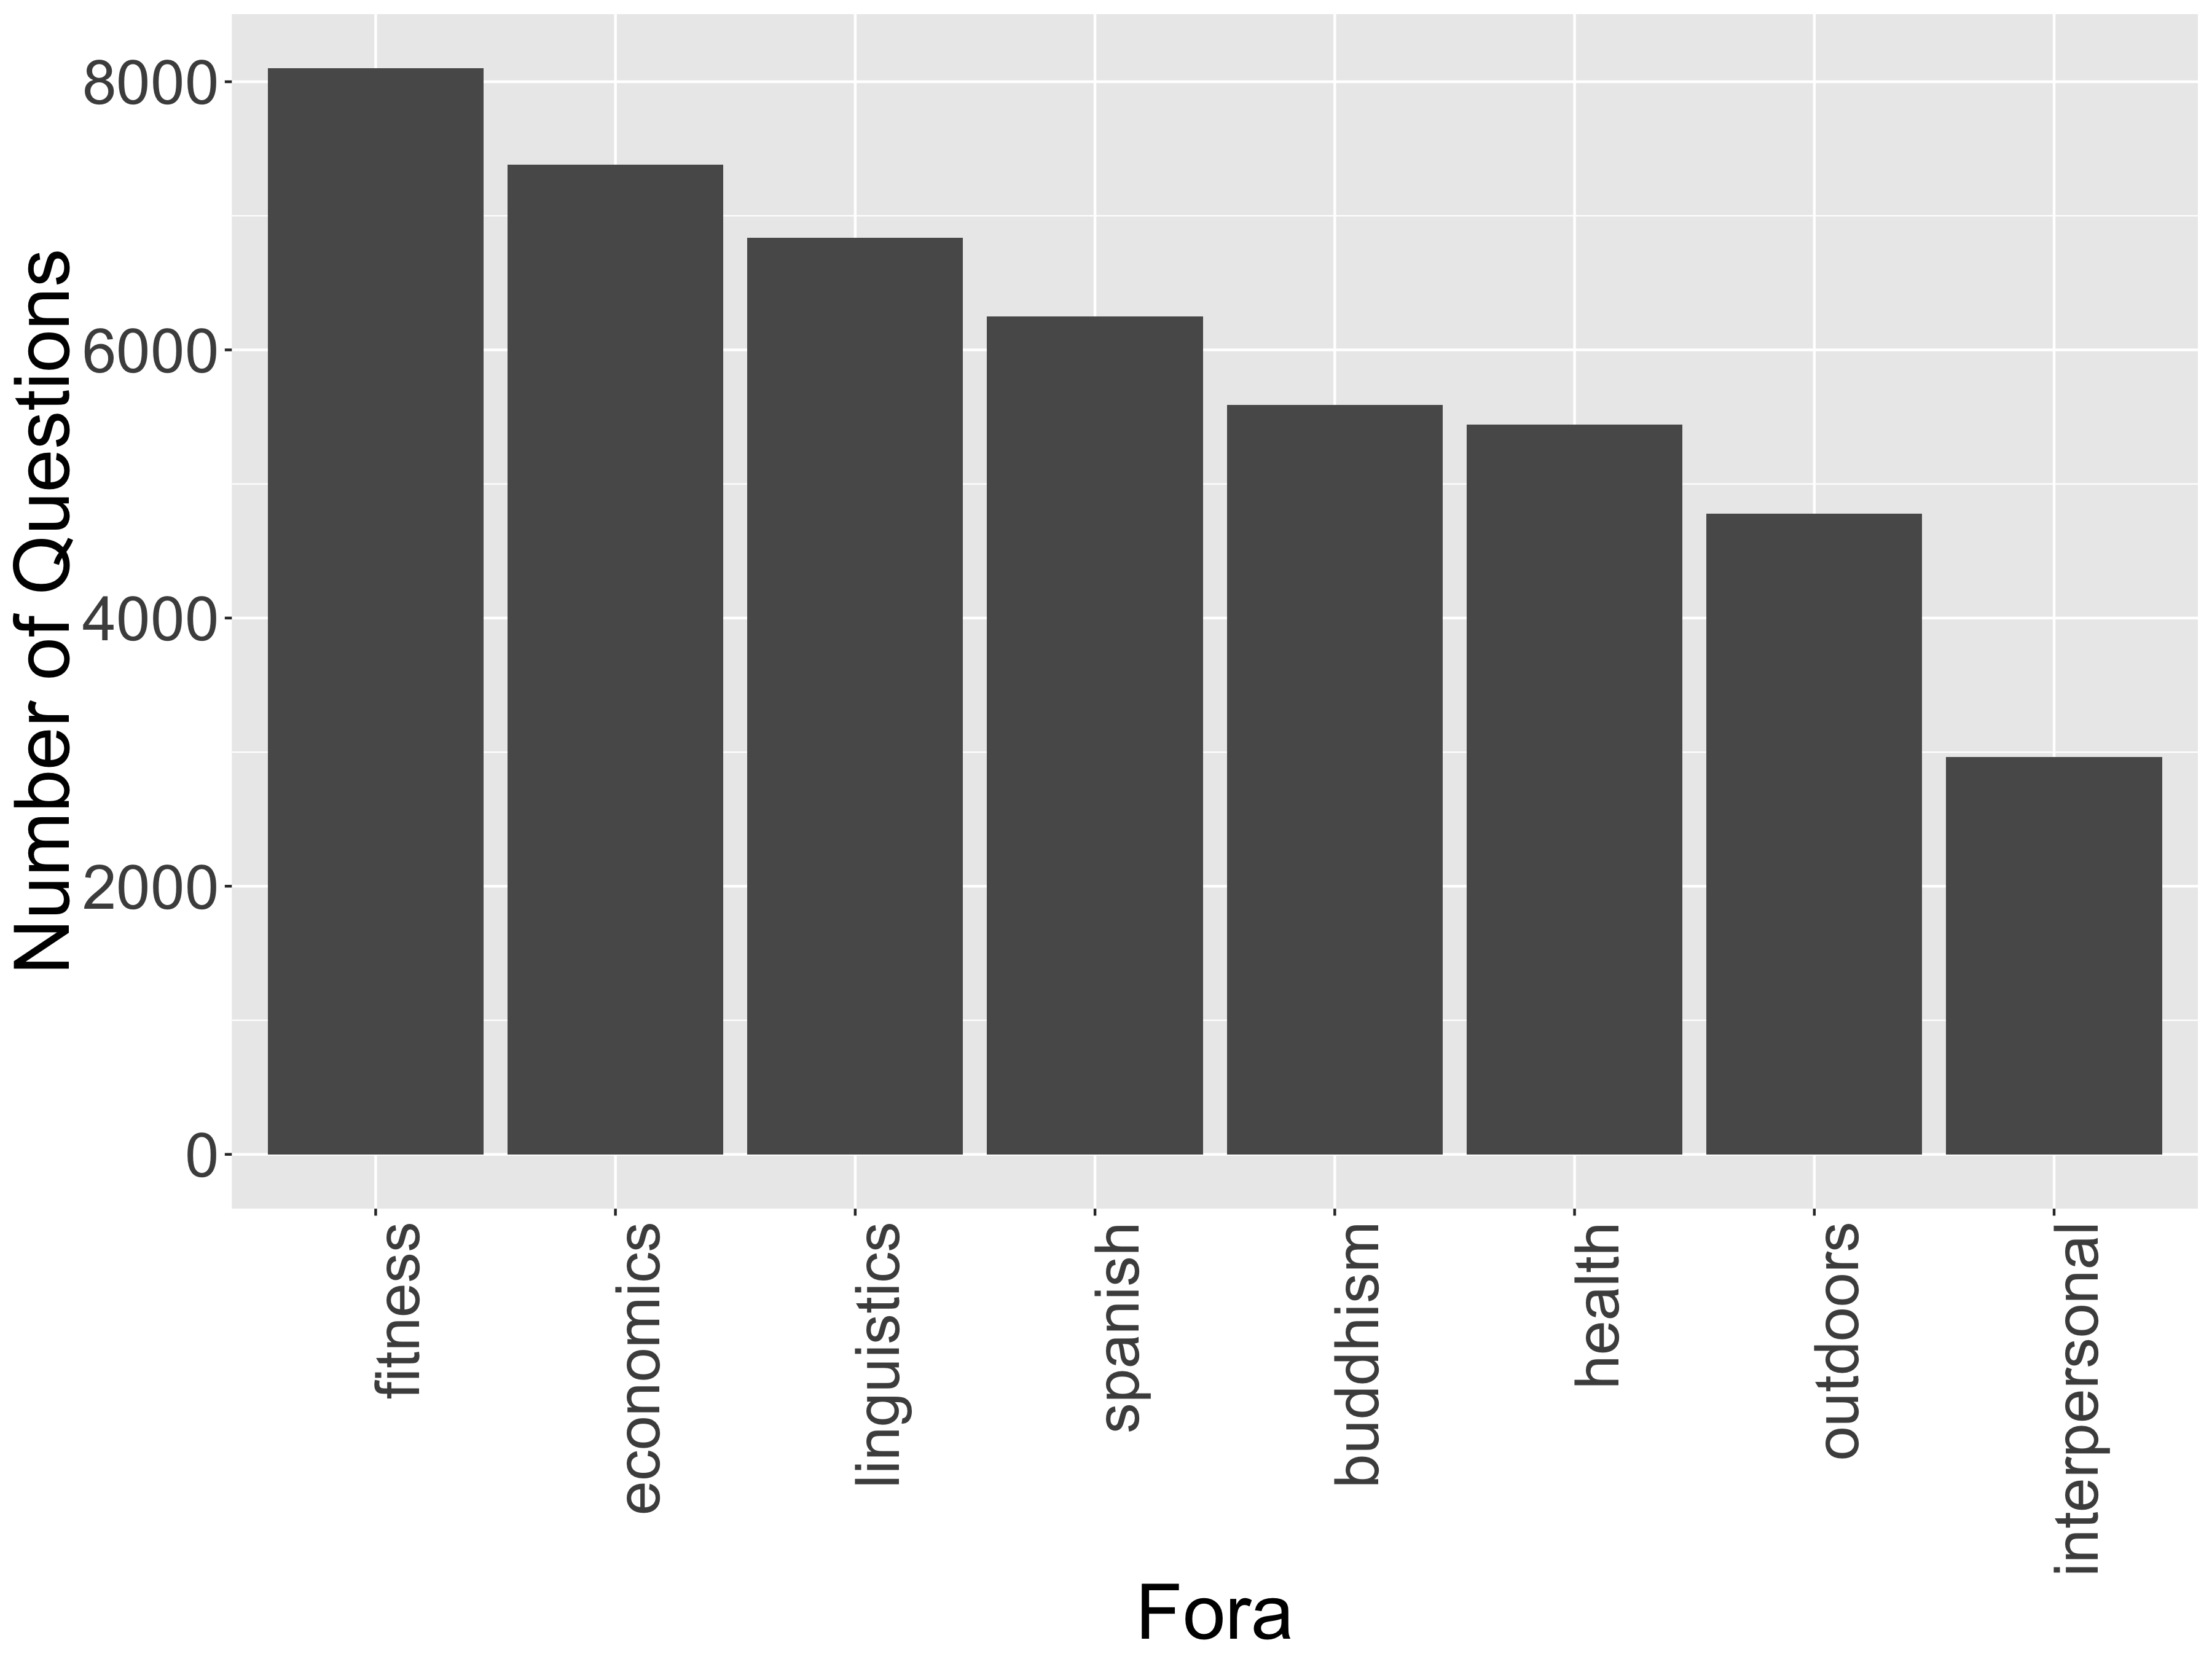
\includegraphics[width=0.5\linewidth]{./results/q-count-bar-graph} \end{center}



\begin{center}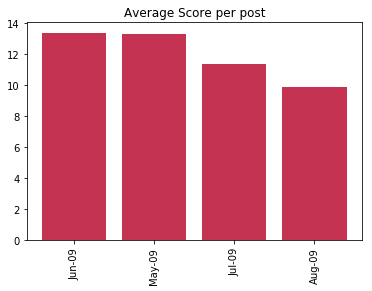
\includegraphics[width=0.5\linewidth]{./results/ave-score-bar-graph} \end{center}



\begin{center}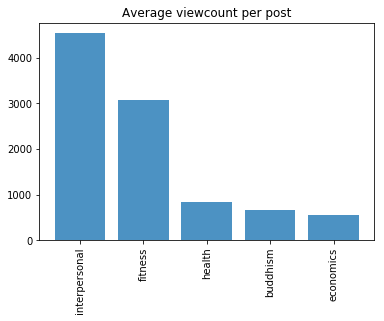
\includegraphics[width=0.5\linewidth]{./results/ave-views-bar-graph} \end{center}
\centering
{\footnotesize Source: Own calculations in R.}
\end{figure}

\normalsize

\begin{figure}
\caption{\textbf{Cumulative Graph for Question Viewcounts}}
\label{fig:cumul}

\begin{center}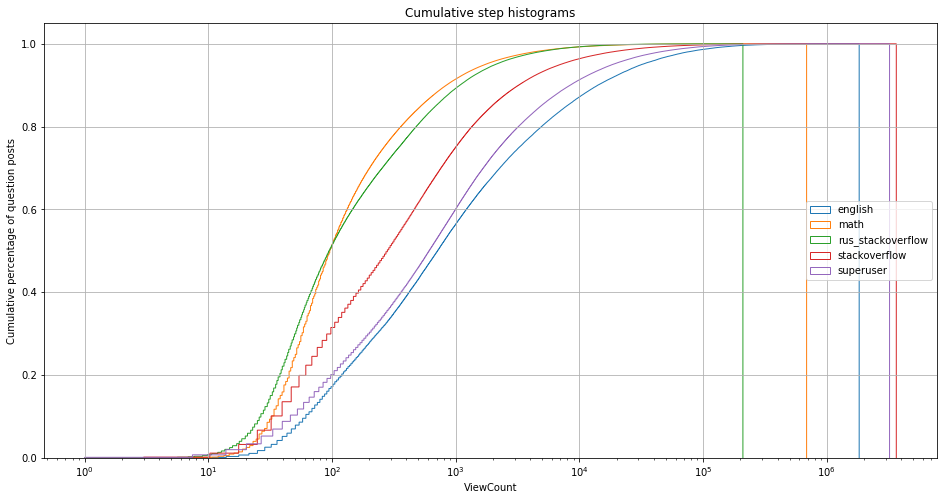
\includegraphics[width=1\linewidth]{./results/cumul-viewcount} \end{center}
\centering
{\footnotesize Source: Own calculations in R.}
\end{figure}

\normalsize

Figure \ref{fig:cumul} plots cumulative percentages of questions as a
function of \texttt{ViewCount} in each fora. There are two aspects of
the graph that are noteworthy - the order of the curves from left to
right, and the fact that they maintain this order (i.e.~they are roughly
parallel). The further right a curve is is indicative of high
\texttt{ViewCounts} per post overall, and we see that this does mirror
the averages calculated in the \texttt{ViewCount} descriptive bar graph
in figure \ref{fig:desc}.

A crossing of curves in figure \ref{fig:cumul} would indicate that there
are certain \texttt{ViewCount} thresholds where a forum becomes more
popular (experiences more viewing traffic) than another. Since there is
very little crossing of curves over all fora, if at all, it appears as
though the distribution of \texttt{ViewCount} across fora is fairly
homogeneous and has relatively constant variance.

\section{Methodology}\label{methodology}

\subsection{\texorpdfstring{The \texttt{Score}
Variable}{The Score Variable}}\label{the-score-variable}

Now that I have parsed question content for the fora in the
\texttt{Body} variable, I move onto defining a metric that measures
community engagement. As previously mentioned, I choose the same metric
used in Ravi \emph{et al.} (2014), a question's \texttt{Score} to
measure what I consider community engagement for questions. A point of
departure here however, is that Ravi \emph{et al.} (2014) choose to
eliminate questions below a certain \texttt{ViewCount} threshold to
control for the possibility that sufficient users
qualified\footnote{See section 4.2 for a discussion on registered user privileges}
to vote do not see these questions.

I feel that while it may partly be random chance that these questions do
not receive views from qualified users, there may also be inherent
qualities and aspects of these questions that explain this occurrence,
and thus they should be incorporated into the final prediction model
since this is precisely a case of a lack of community engagement. I
therefore do not discard any questions from the fora.

A pertinent finding from Ravi \emph{et al.} (2014) is that questions
with higher \texttt{ViewCounts} are more likely to receive higher
\texttt{Scores}. They consequently normalise \texttt{Score} by
\texttt{ViewCount} to mitigate the possibility of conflating popularity
with what they assume is question quality. I replicate this step in
their methodology, and table \ref{tab:bestworst} displays the titles of
a selection of ``best'' and ``worst'' questions across fora according to
the final response variable \texttt{Score}/\texttt{ViewCount} (the best
questions have positive \texttt{Scores} whereas the worst have negative
\texttt{Scores}).

Table \ref{tab:bestworst} appears to show that questions that are
considered the ``best'' tend to be honest and discussion-promoting,
whereas the ``worst'' questions are often sarcastic and probably not
genuinely looking for an answer - the questions from the Economics and
Fitness fora illustrate this. Social norms also appear to play a strong
part, since the ``worst'' question on the Interpersonal forum eludes to
children being unvaccinated, which I assume would upset many individuals
on the forum and lead to lowest \texttt{Score} per \texttt{ViewCount}
for that forum.

\newpage

\setcounter{table}{1} \footnotesize

\begin{longtable} {@{} cccp{11cm} @{}}
\caption{\textbf{Best and Worst Fora Questions According to Score/ViewCount}}
\label{tab:bestworst}\\ \hline \hline
\textbf{Forum} & \textbf{Score} & \textbf{ViewCount} & \textbf{Title} \\ 
\hline
Buddhism & 13 & 176 & What are the texts that contain words which can be attributed directly to the Buddha? \\
\hline
Economics & -9 & 102 & Has anyone made a successful economic prediction more than once? \\
\hline
Health & 14 & 95 & In which order to put on a mask, a gown and to disinfect when visiting a hospital patient? \\ 
\hline
Fitness & -5 & 201 & What is the best way to gain size in ankle area \\ 
\hline
Interpersonal & 24 & 1054 & How can I notice if someone is speaking with sarcasm or irony? \\ 
\hline
Interpersonal & -9 & 1327 & How can I tell if family members consider my unvaccinated kids a threat? \\ 
\hline
Spanish & 20 & 330 & Is the use of @ instead of 'a' or 'o' in order to refer to both masculine and femenine accepted? \\ 
\hline \hline
\end{longtable}\begin{center} Source: Own calculations in R.\end{center}

\normalsize

\subsection{Final Binary Response
Variable}\label{final-binary-response-variable}

For the purpose of predicting in the classification model, Ravi \emph{et
al.} (2014) decide on a binary response i.e.~labeling questions as only
``good'' versus
``bad''\footnote{For clarity, when referring to good and bad questions in this research, I refer to questions being able to attract positive and negative community engagement}.
This clearly ignores the fact that community engagement lies on a
spectrum, but it simplifies the prediction step and thus I emulate this
and leave it up to further research to predict on a range of community
engagement.

The crucial issue at this stage is that Ravi \emph{et al.} (2014) decide
on a decision boundary of 0.001 for the
\texttt{Score}/\texttt{ViewCount} response variable, above which they
define good questions, and below bad questions. Other than stating that
their reason for this is so that they are ``confident that this reflects
the good quality of {[}a question{]}, rather than an incidental click on
the up vote'', the full motivation behind why this specific bound was
chosen over others appears to be lacking.

This is not a trivial decision, since in selecting a bound one makes a
strong assumption on what the ratio of good and bad questions is for a
given community. This is exacerbated by the fact that the response is
now binary, since questions that are on the margin and are barely
labeled ``good'' will be treated the same as the ``best'' questions in
the final prediction model. It is at this key step that I perform
validation checks to shed light on what the optimal choice is.

\newpage

\section{Results}\label{results}

The boundary of 0.001 for the \texttt{Score}/\texttt{ViewCount} variable
used in Ravi \emph{et al.} (2014) appears to be half of the mean for the
variable - my investigations found that this results in approximately
60\% of questions being labeled as ``good'' in the data, therefore I use
this as the baseline comparison among other
thresholds\footnote{Again in the interest of clarity, when I refer to threshold I am referring to the percentage of questions labeled "good"}
in these results.

I compare the splitting of good/bad questions on a threshold using
Cosine and Jaccard
similarity\footnote{Euclidean distance was not included owing to it capturing essentially the same information as Cosine similarity}
with the assumption being that good and bad questions will differ across
these metrics owing to differences in their feature use. For each
threshold tested, document feature matrices were constructed (weighted,
stemmed, with no stopwords or punctuation) on both samples of good- and
bad-labeled questions to calculate the similarity statistics using the
\texttt{textstat\_simil} function from the \texttt{quanteda} package.

For thresholds between 0\% and 50\% I compare symmetric samples -
i.e.~for a threshold of 10\% corresponding to the 10\% ``best''
questions (a high decision boundary for the
\texttt{Score}/\texttt{ViewCount} variable) I compare the ``worst'' 10\%
of questions. In this way, questions symmetrically around the 50\% mark
are ignored until the 50\% threshold is reached. Past the 50\% mark I
compare all questions labeled good with all questions labeled bad,
i.e.~a threshold of 60\% would be compared the other 40\% questions
labeled bad.

Figure \ref{fig:simil} plots how the two similarity metrics vary over
the different thresholds. Low values for these graphs indicate low
similarity and thus higher distinction between good/bad samples, and the
black vertical line is the 60\% baseline comparison. The curves across
both graphs are roughly inverted-U-shaped and similar to one another,
indicating the disparity between the very ``best'' and ``worst''
questions on the far left, and on the far right showing that the very
``worst'' questions differ substantially from the rest of the corpus.

In both graphs on the far left we see significant oscillation of the
curves - this is most likely a result of subsets of the data being
compared rather than the full corpus. The low similarities of around
0.85-0.925 for the Economics, Fitness and Linguistics fora in the Cosine
similarity plot are expected, since the very best and worst questions
are being compared here. What is interesting is that not all of the
curves in the Cosine similarity graph depict this expected behaviour,
with some fora like Outdoors almost having a negative slope for the
entire range of thresholds.

\setcounter{figure}{2}

\begin{figure}
\caption{\textbf{Comparing Feature Use Across Good and Bad Questions}}
\label{fig:simil}

\begin{center}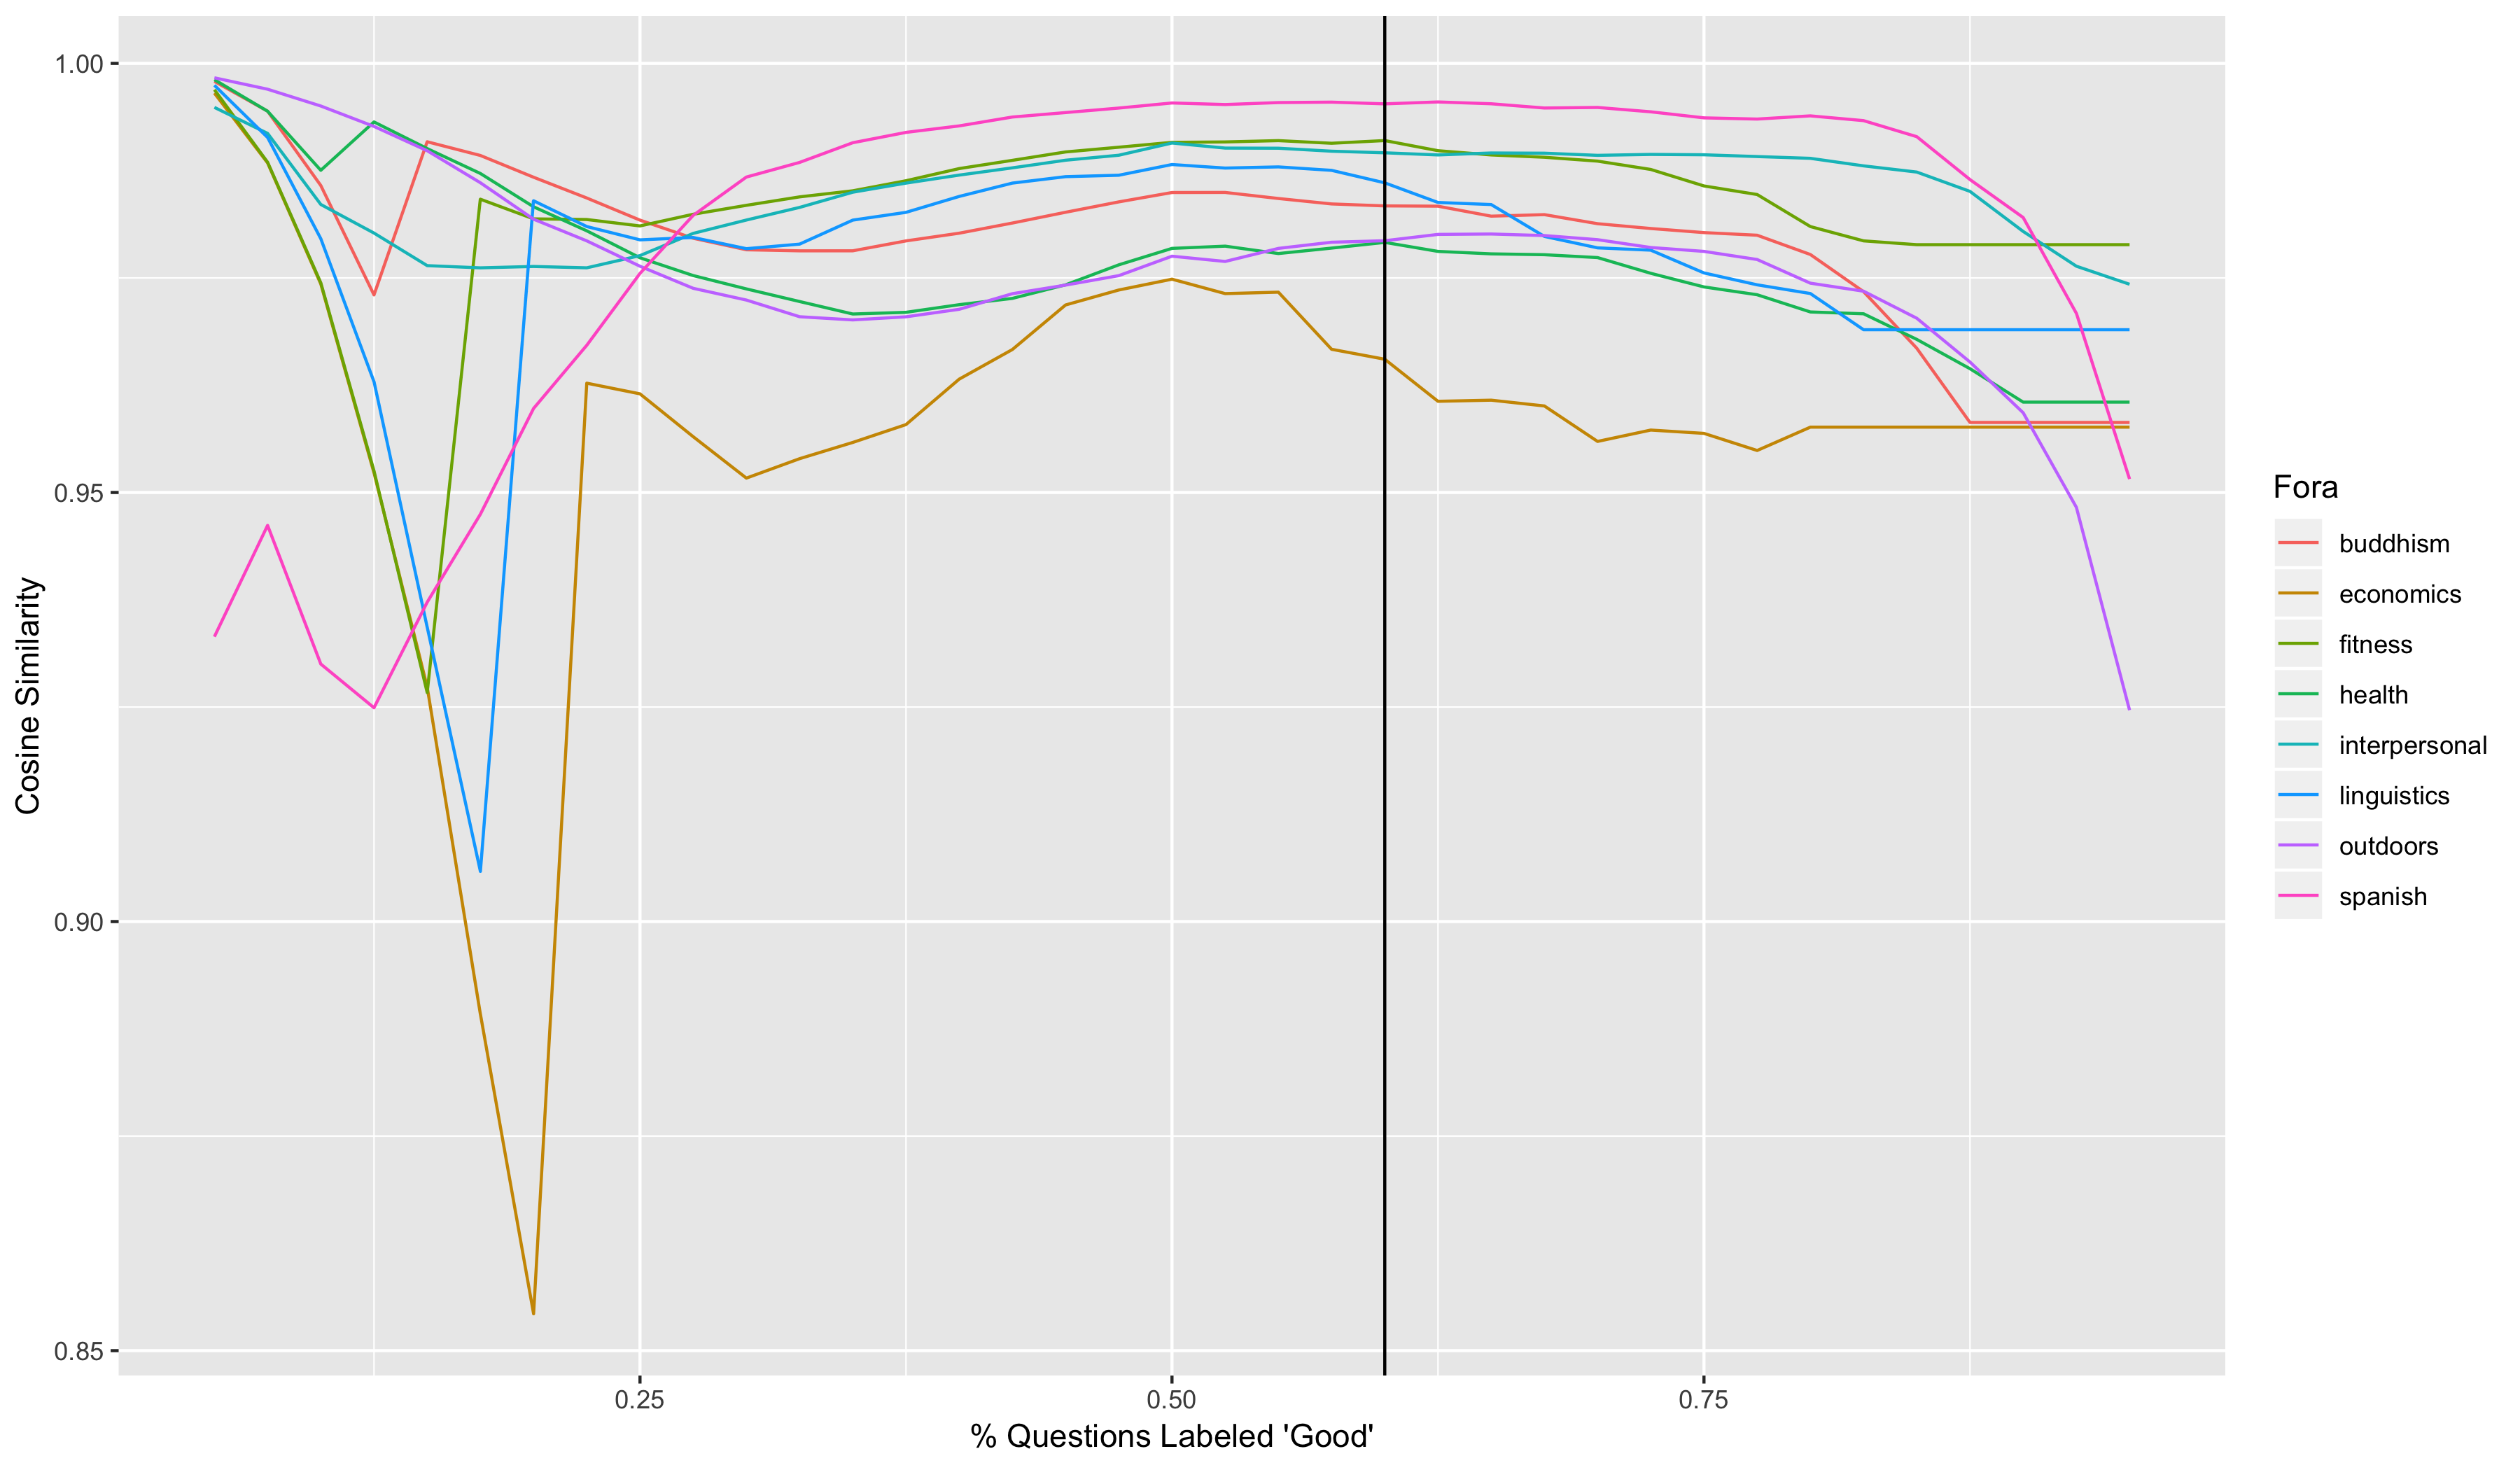
\includegraphics[width=1\linewidth]{./results/threshold-cos} \end{center}



\begin{center}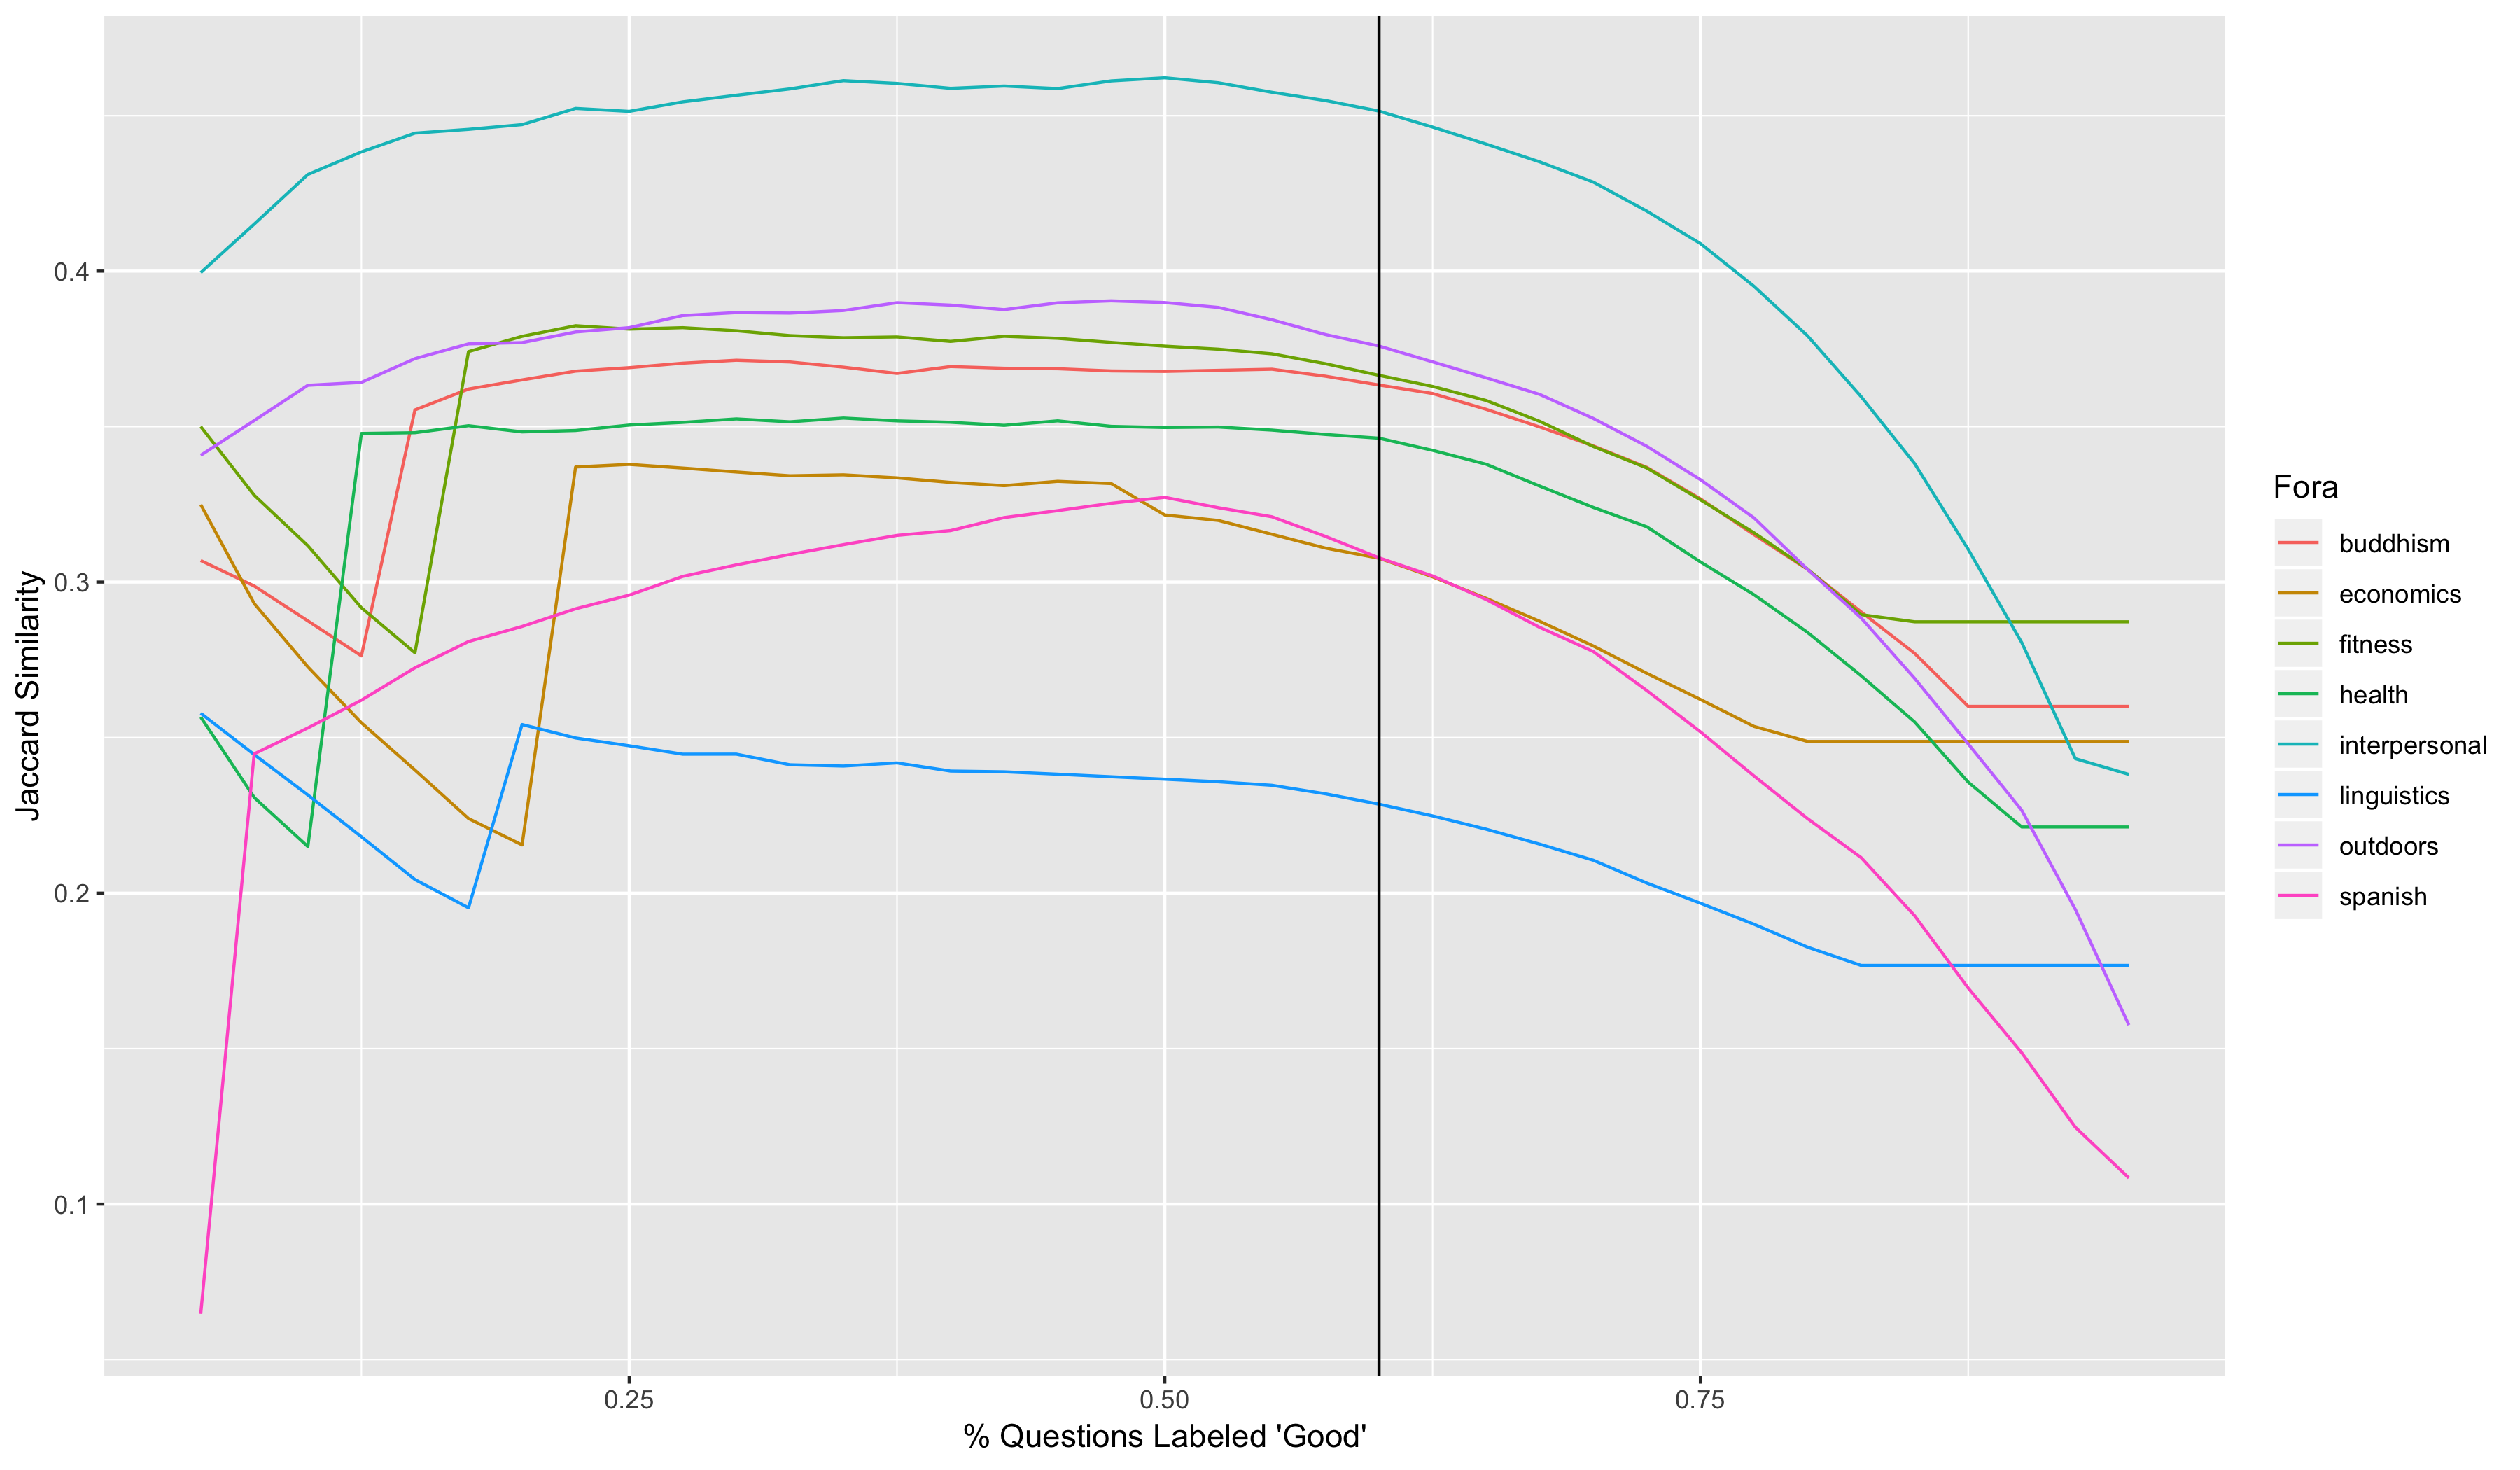
\includegraphics[width=1\linewidth]{./results/threshold-jac} \end{center}
\centering
{\footnotesize Source: Own calculations in R.}
\end{figure}

\normalsize

Most interestingly, all curves across both graphs appear to converge
towards each other and in shape from a 30\% threshold onward. The fact
that some curves even plateau and reach local minima after tapering off
on the far right indicates not only that higher thresholds
(\textgreater{} 50\%) lead to more distinct good/bad samples (which
wasn't unexpected), but that an optimal threshold could be achieved
where the samples are distinct and there is still a substantial number
of bad-labeled questions.

Keeping in mind that the threshold decision necessitates an assumption
of what the ratio of bad and good questions are in fora, I finally
perform difference-of-means tests across other linguistics features for
the Interpersonal and
Economics\footnote{The results of only two fora are presented for the sake of brevity}
fora with thresholds of 80\% and 75\% respectively. Once again, the main
assumption here is that good and bad questions differ across the
features measured. The results are displayed in tables
\ref{tab:pers_stat} and \ref{tab:ecos_stat}, with statistical
significance for differences displayed for character length up to moral
values\footnote{The Wilcoxon Rank Sum Test is used owing to it being non-parametric and thus not assuming a distributional form for the data}.
\newline

\setcounter{table}{2}

\footnotesize

\begin{longtable} {@{} c|ccc|ccc @{}}
\caption{\textbf{Interpersonal Linguistic Statistical Differences}}
\label{tab:pers_stat}\\ \hline \hline
 & \multicolumn{3}{c}{60\% Good Questions} & \multicolumn{3}{c}{80\% Good Questions}  \\ 
Metric & Good & Bad & Diff. & Good & Bad & Diff. \\ 
\hline \\[-1.8ex] 
N & 1777.00 & 1185.00 & 592 & 2369.00 &  593.00 & 1776 \\ 
N\% &   59.99 &   40.01 & 19.99 &   79.98 &   20.02 & 59.96 \\ 
Punctuation Types &   36.00 &   42.00 & -6 &   41.00 &   36.00 & 5 \\ 
URL-Text Types &   28.00 &   25.00 & 3 &   49.00 &    0.00 & 49 \\ 
Stopword Types &  346.00 &  341.00 & 5 &  357.00 &  314.00 & 43 \\ 
\hline
Character Length & 1636.95 & 1774.04 & -137.09\textasteriskcentered \textasteriskcentered  & 1690.81 & 1695.74 & -4.93 \\ 
Token Length &  337.01 &  368.06 & -31.06\textasteriskcentered \textasteriskcentered \textasteriskcentered  &  348.66 &  352.53 & -3.87 \\ 
Guiraud's Root TTR &    8.83 &    8.87 & -0.04 &    8.89 &    8.68 & 0.21\textasteriskcentered \textasteriskcentered \textasteriskcentered  \\ 
Yule's K &  158.90 &  158.44 & 0.46 &  157.27 &  164.50 & -7.23\textasteriskcentered \textasteriskcentered  \\ 
Flesch-Kincaid &    9.35 &    9.14 & 0.2\textasteriskcentered \textasteriskcentered  &    9.29 &    9.14 & 0.15\textasteriskcentered \textasteriskcentered  \\ 
Gunning's Fog Index &   12.18 &   11.92 & 0.26\textasteriskcentered \textasteriskcentered \textasteriskcentered  &   12.12 &   11.90 & 0.22\textasteriskcentered \textasteriskcentered \textasteriskcentered  \\ 
Sentiment &    0.22 &    0.21 & 0.01 &    0.22 &    0.22 & 0 \\ 
Moral Values &    0.55 &    0.51 & 0.04\textasteriskcentered  &    0.54 &    0.51 & 0.03 \\ 
\hline \hline
\multicolumn{7}{l}{Note: Wilcoxon Rank Sum Test statistical significance represented at the 0.05,} \\
\multicolumn{7}{l}{ 0.01 and 0.001 level by *, ** and *** respectively.} \\
\multicolumn{7}{l}{Source: Own calculations in R.}\\
\end{longtable}

\normalsize

There are a number of noteworthy results from table \ref{tab:pers_stat}
for the Interpersonal forum. The first is that the new threshold has
resulted in starker differences for some linguistic features, but not
for others. This hints that our assumption of distinctions necessarily
existing across all features between samples may be incorrect.

Secondly, the split for the new threshold results in a good-sample that
uses far greater selections of URL-text, stopwords and punctuation. This
implies that the new threshold is separating out questions that are more
linguistically complex and potentially show more prior research (by
linking URLs in the question \texttt{Body}). This is confirmed by the
larger differences of lexical complexity (Guiraud's Root TTR and Yule's
K) for the new threshold, now also both statistically significant at the
0.001 level. Lastly, the difference in character/word lengths and
appeal-to-moral-values of good/bad questions has diminished for the new
threshold, whereas the results for readability (Flesch-Kincaid and
Gunning's Fog Index) and sentiment are essentially the same for both
thresholds.

\footnotesize

\begin{longtable}[htbp] {@{} c|ccc|ccc @{}}
\caption{\textbf{Economics Linguistic Statistical Differences}}
\label{tab:ecos_stat}\\ \hline \hline
 & \multicolumn{3}{c}{60\% Good Questions} & \multicolumn{3}{c}{75\% Good Questions}  \\ 
Metric & Good & Bad & Diff. & Good & Bad & Diff. \\ 
\hline \\[-1.8ex] 
N & 4428.00 & 2952.00 & 1476 & 5535.00 & 1845.00 & 3690 \\ 
N\% &   60.00 &   40.00 & 20 &   75.00 &   25.00 & 50 \\ 
Punctuation Types &   86.00 &   86.00 & 0 &   94.00 &   73.00 & 21 \\ 
URL-Text Types &  577.00 &  390.00 & 187 &  707.00 &  243.00 & 464 \\ 
Stopword Types &  346.00 &  334.00 & 12 &  356.00 &  315.00 & 41 \\ 
\hline
Character Length &  841.03 &  705.12 & 135.91\textasteriskcentered \textasteriskcentered \textasteriskcentered  &  835.84 &  639.16 & 196.67\textasteriskcentered \textasteriskcentered \textasteriskcentered  \\ 
Token Length &  189.00 &  153.83 & 35.17\textasteriskcentered \textasteriskcentered \textasteriskcentered  &  187.59 &  136.98 & 50.61\textasteriskcentered \textasteriskcentered \textasteriskcentered  \\ 
Guiraud's Root TTR &    6.71 &    6.29 & 0.42\textasteriskcentered \textasteriskcentered \textasteriskcentered  &    6.67 &    6.16 & 0.52\textasteriskcentered \textasteriskcentered \textasteriskcentered  \\ 
Yule's K &  261.48 &  299.75 & -38.27\textasteriskcentered \textasteriskcentered \textasteriskcentered  &  264.80 &  312.76 & -47.97\textasteriskcentered \textasteriskcentered \textasteriskcentered  \\ 
Flesch-Kincaid &   11.58 &   10.95 & 0.63\textasteriskcentered \textasteriskcentered \textasteriskcentered  &   11.50 &   10.81 & 0.7\textasteriskcentered \textasteriskcentered \textasteriskcentered  \\ 
Gunning's Fog Index &   14.86 &   14.25 & 0.61\textasteriskcentered \textasteriskcentered \textasteriskcentered  &   14.79 &   14.09 & 0.7\textasteriskcentered \textasteriskcentered \textasteriskcentered  \\ 
Sentiment &    0.24 &    0.22 & 0.02\textasteriskcentered  &    0.24 &    0.22 & 0.03\textasteriskcentered \textasteriskcentered  \\ 
Moral Values &    0.48 &    0.44 & 0.04\textasteriskcentered \textasteriskcentered \textasteriskcentered  &    0.47 &    0.45 & 0.03\textasteriskcentered \textasteriskcentered  \\ 
\hline \hline
\multicolumn{7}{l}{Note: Wilcoxon Rank Sum Test statistical significance represented at the 0.05,} \\
\multicolumn{7}{l}{ 0.01 and 0.001 level by *, ** and *** respectively.} \\
\multicolumn{7}{l}{Source: Own calculations in R.}\\
\end{longtable}

\normalsize

\newpage

For the results of the Economics forum in table \ref{tab:ecos_stat},
there are in fact greater differences across all metrics with
approximately the same statistical significance results. This is
substantial evidence that a threshold of 75\% results in higher
discernment between good and bad question samples, while still
maintaining at least a quarter of questions labeled as bad. Overall, the
results above indicate that unique and optimal thresholds can be
investigated and implemented across all fora, providing more robust
binary samples for prediction and classification of community
engagement.

\section{\texorpdfstring{Conclusion
\label{Concl}}{Conclusion }}\label{conclusion}

The discussion and results of this paper demonstrate that the decision
on where to label good and bad questions for online question-answer
communities using the \texttt{Score}/\texttt{ViewCount} variable, or any
response variable for that matter, should not be taken lightly. By
analysing the distinguishing linguistic factors of various thresholds of
good-labeled questions, I was able to establish that more optimal
decision boundaries can be obtained for this variable in the interest of
more robustly capturing and predicting positive community engagement.

It is recommended that future research analyse further Q\&A community
data and particularly the StackOverflow forum used in Ravi \emph{et al.}
(2014) in order to ascertain how their threshold compares to potentially
more optimal values. Further work could also attempt to capture and
predict on a range of community engagement rather than the discrete
binary response defined in this paper.

One area of further research that I plan to pursue is to take these
results and implement them in a binary classification model of my own,
with the aim of predicting questions that elicit positive community
engagement. In this way, I hope to assist online Q\&A fora users in
improving their questions, and consequently improve the prosperity of
online Q\&A communities as a whole.

\newpage

\section*{References}\label{references}
\addcontentsline{toc}{section}{References}

\hypertarget{refs}{}
\hypertarget{ref-Agichtein2008}{}
Agichtein, E. \emph{et al.} (2008) `Finding high-quality content in
social media', in \emph{Proceedings of the 2008 international conference
on web search and data mining}. ACM, pp. 183--194. doi:
\href{https://doi.org/10.1145/1341531.1341557}{10.1145/1341531.1341557}.

\hypertarget{ref-Berry2017}{}
Berry, G. and Taylor, S. J. (2017) `Discussion quality diffuses in the
digital public square'. Available at:
\url{http://arxiv.org/abs/1702.06677}.

\hypertarget{ref-Bian2009}{}
Bian, J. \emph{et al.} (2009) `Learning to recognize reliable users and
content in social media with coupled mutual reinforcement', in
\emph{Proceedings of the 18th international conference on world wide
web}. ACM, pp. 51--60. doi:
\href{https://doi.org/10.1145/1526709.1526717}{10.1145/1526709.1526717}.

\hypertarget{ref-Gervais2015}{}
Gervais, B. T. (2015) `Incivility Online: Affective and Behavioral
Reactions to Uncivil Political Posts in a Web-based Experiment'. doi:
\href{https://doi.org/10.1080/19331681.2014.997416}{10.1080/19331681.2014.997416}.

\hypertarget{ref-Jeon2006}{}
Jeon, J. \emph{et al.} (2006) `A framework to predict the quality of
answers with non-textual features', in \emph{Proceedings of the 29th
annual international acm sigir conference on research and development in
information retrieval}. ACM, pp. 228--235. doi:
\href{https://doi.org/10.1145/1148170.1148212}{10.1145/1148170.1148212}.

\hypertarget{ref-Li2010}{}
Li, B. and King, I. (2010) `Routing questions to appropriate answerers
in community question answering services', in \emph{Proceedings of the
19th acm international conference on information and knowledge
management}. ACM, pp. 1585--1588. doi:
\href{https://doi.org/10.1145/1871437.1871678}{10.1145/1871437.1871678}.

\hypertarget{ref-Li2012}{}
Li, B. \emph{et al.} (2012) `Analyzing and predicting question quality
in community question answering services', in \emph{Proceedings of the
21st international conference on world wide web}. ACM, pp. 775--782.
doi:
\href{https://doi.org/10.1145/2187980.2188200}{10.1145/2187980.2188200}.

\hypertarget{ref-Li2011}{}
Li, B., King, I. and Lyu, M. R. (2011) `Question routing in community
question answering', in \emph{Proceedings of the 20th acm international
conference on information and knowledge management}. ACM, pp.
2041--2044. doi:
\href{https://doi.org/10.1145/2063576.2063885}{10.1145/2063576.2063885}.

\hypertarget{ref-Liu2008}{}
Liu, Y., Bian, J. and Agichtein, E. (2008) `Predicting information
seeker satisfaction in community question answering', in
\emph{Proceedings of the 31st annual international acm sigir conference
on research and development in information retrieval}. ACM (Section 2),
pp. 483--490. doi:
\href{https://doi.org/10.1145/1390334.1390417}{10.1145/1390334.1390417}.

\hypertarget{ref-Qu2009}{}
Qu, M. \emph{et al.} (2009) `Probabilistic question recommendation for
question answering communities', in \emph{Proceedings of the 18th
international conference on world wide web}. ACM (2), pp. 1229--1230.
doi:
\href{https://doi.org/10.1145/1526709.1526942}{10.1145/1526709.1526942}.

\hypertarget{ref-Ravi2014}{}
Ravi, S. \emph{et al.} (2014) `Great Question! Question Quality in
Community Q\&A.', in \emph{Eighth international aaai conference on
weblogs and social media}. (1), pp. 426--435.

\hypertarget{ref-Riahi2012}{}
Riahi, F. \emph{et al.} (2012) `Finding expert users in community
question answering', in \emph{Proceedings of the 21st international
conference on world wide web}. ACM, pp. 791--798. doi:
\href{https://doi.org/10.1145/2187980.2188202}{10.1145/2187980.2188202}.

\hypertarget{ref-Shah2010}{}
Shah, C. and Pomerantz, J. (2010) `Evaluating and predicting answer
quality in community QA', in \emph{Proceedings of the 33rd international
acm sigir conference on research and development in information
retrieval}. ACM (March 2008), pp. 411--418. doi:
\href{https://doi.org/10.1145/1835449.1835518}{10.1145/1835449.1835518}.

\hypertarget{ref-Shah2018}{}
Shah, V. \emph{et al.} (2018) `Adaptive matching for expert systems with
uncertain task types', in \emph{2017 55th annual allerton conference on
communication, control, and computing (allerton)}. IEEE, pp. 753--760.
doi:
\href{https://doi.org/10.1109/ALLERTON.2017.8262814}{10.1109/ALLERTON.2017.8262814}.

\hypertarget{ref-Sung2013}{}
Sung, J., Lee, J.-g. and Lee, U. (2013) `Booming Up the Long Tails:
Discovering Potentially Contributive Users in Community-Based Question
Answering Services', in \emph{Seventh international aaai conference on
weblogs and social media}, pp. 602--610.

\hypertarget{ref-Szpektor2013}{}
Szpektor, I., Maarek, Y. and Pelleg, D. (2013) `When relevance is not
enough: promoting diversity and freshness in personalized question
recommendation', in \emph{Proceedings of the 22nd international
conference on world wide web}. ACM, pp. 1249--1260.

\hypertarget{ref-Tian2013}{}
Tian, Q., Zhang, P. and Li, B. (2013) `Towards Predicting the Best
Answers in Community-Based Question-Answering Services', in
\emph{Seventh international aaai conference on weblogs and social
media}, pp. 725--728.

\hypertarget{ref-Wu2008}{}
Wu, H., Wang, Y. and Cheng, X. (2008) `Incremental probabilistic latent
semantic analysis for automatic question recommendation', in
\emph{Proceedings of the 2008 acm conference on recommender systems}.
ACM, p. 99. doi:
\href{https://doi.org/10.1145/1454008.1454026}{10.1145/1454008.1454026}.

\hypertarget{ref-Zhou2012}{}
Zhou, T. C., Lyu, M. R. and King, I. (2012) `A classification-based
approach to question routing in community question answering', in
\emph{Proceedings of the 21st international conference on world wide
web}. ACM, pp. 783--790. Available at:
\url{http://www2012.wwwconference.org/proceedings/companion/p783.pdf}.

\newcommand\wordcount{
    \immediate\write18{texcount -sub=section \jobname.tex  | grep "Section" |     sed -e 's/+.*//' | sed -n \thesection p > 'count.txt'}
(\input{count.txt}words)}

\end{document}
